\documentclass{llncs}
\usepackage[ruled,vlined]{algorithm2e}
\usepackage{color,graphicx,epstopdf,changepage,amsmath,multirow}
\usepackage[justification=centering]{caption}
\SetAlgoCaptionSeparator{.\space}
\renewcommand\AlCapFnt{\normalfont\scshape}
\setlength{\algomargin}{0.7cm}

\title{Comprehensive Quality Awareness Automated Semantic Web Service Composition}
\author{Chen Wang, Hui Ma, and Aaron Chen}
\institute{School of Engineering and Computer Science,
\\Victoria University of Wellington, New Zealand \\
Email: \{chen.wang, hui.ma, aaron.chen\}@ecs.vuw.ac.nz}


\usepackage[pdfauthor={\@author}, pdftitle={\@title}]{hyperref}
\makeatother

%\providecommand{\e}[1]{\ensuremath{\times 10^{#1}}}
\vspace{-1.5cm}

\begin{document}
\maketitle
\begin{abstract}
Semantic web service composition has been a prevailing research area in recent years. There are two major challenges faced by researchers, semantic matchmaking and Quality of Service (QoS) optimisation. Semantic matchmaking aims to discover interoperable web services that can interact with each other to provide rich functionalities through language understanding and reasoning. QoS optimisation aims to optimise the non-functional requirements of service users, e.g., minimum cost, maximal reliability. Many scholars have looked into QoS optimisation problems in QoS-aware web service composition, applying AI planning and Evolutionary Computation techniques. To meet users' requirements, one often needs to consider both semantic matchmaking quality and QoS simultaneously. Existing works on web service composition often concern either semantic web  service composition or QoS-aware web service composition. Therefore, we propose a general comprehensive quality model considering semantic matchmaking quality and QoS simultaneously that can achieve a more desirable trade-off in consideration of both sides. Further more, we develop a PSO-based service composition approach with explicit support for the comprehensive model. We compare this model with a promising QoS-aware model, and also compare our PSO-based method with one recent GP-based method to show its performance in finding a more optimised solution.

\end{abstract}
\section{Introduction}\label{introduction}

\textit{Web service composition} pertains to a combination of multiple web services to provide a value-added composition service that accommodates customers' arbitrarily complex requirements. This application is developed by integrating interoperable and collaborative functionalities over heterogeneous systems. Due to the increasing number of large-scale enterprise applications, the number of Web services has increased substantially and unprecedentedly. Therefore, manual and semi-automated web service compositions are considered to be less efficient while automated web service composition has less human intervention, less time consumption, and high productivity.

Two most notable challenges for web service composition are ensuring interoperability of services and achieving Quality of Service (QoS) optimisation \cite{fensel2011semantic}. \textit{Interoperability} of web services presents challenge in syntactic and semantic dimensions. The syntactic dimension is covered by the XML-based technologies (such as $WSDL$, $SOAP$). The semantic aspect, on the other hand, demands further research. Through ontology-based semantics \cite{o2005review}, web services can understand and better collaborate with each other. There are many ontology languages and formats for semantic service descriptions, such as OWL-S, WSML, and SAWSDL \cite{petrie2016web}, which make ``machine understanding'' possible through identifying and matching semantic similarities in input/output parameters of web services in heterogeneous environments. The second challenge $(2)$ is related to finding \textit{optimised solutions} to QoS. This problem gives birth to \textit{QoS-aware service composition} that considers the composition of service-level agreements (SLA) \cite {sahai2002automated} involving a collection of SLA rules and policies for supporting QoS-based composition.

Existing works on service composition focus mainly on addressing one of challenges above. Many works have been conducted to optimise the quality of compositions under a pre-defined abstract workflow, which is generally considered as a \textit{semi-automated Web service composition} approach \cite{bahadori2009optimal,parejo2008qos}. Meanwhile, many research works consider the possibility of generating a composition plan automatically in discovering and selecting suitable web services, which are considered to be NP-hard \cite{moghaddam2014service}. \textit{Semantic web services composition} is distinguished from the syntactic service composition, which supplements well defined semantic descriptions from the concept of ontologies, instead of parameters value. In the past few years, substantial works have been done on semantic web service composition \cite{bansal2016generalized,boustil2014semantic,mier2015integrated}. However, few works have enabled truely automatic semantic web service composition, where both QoS and quality of semantic match making will be optimised simultaneously and achieved a desired balance.

The overall goal of this paper is to \textit{develop a general comprehensive approach to automated QoS-aware semantic web service composition that satisfactorily optimises both QoS and semantic matchmaking quality}. Particularly, this paper extends existing works of QoS-aware service composition by considering both QoS optimisation and semantic matchmaking quality optimisation in our proposed comprehensive quality model. Particle Swarm Optimisation (PSO) has shown its promise in searching for near-optimised service composition solutions \cite{da2016particle}. We will propose a PSO-based service composition approach with explicit support for our proposed quality model. We will achieve three objectives in this work as follows:

\begin{enumerate}
 \item To propose a general comprehensive quality model that addresses QoS and semantic matchmaking quality in considering different matching types with corresponding concept similarities.
  
 \item To propose a PSO-based service composition algorithm that utilises the proposed quality model. To do that we will first propose a representation of semantic service composition, which can model the quality of semantic matchmaking and QoS together.
  
 \item To evaluate our proposed approach, we conduct experiments to compare our comprehensive quality model with one widely used QoS evaluation model. We also compare one recent GP approach \cite{ma2015hybrid} with our PSO-based approach using our proposed model. Both comparisons utilise benchmark datasets from Web Services Challenge 2009 (WSC09) \cite{kona2009wsc} 
  
\end{enumerate}

\section{Related Work} \label{relatedWork}
Substantial works on web service composition focus on either semantic web service composition \cite{boustil2014semantic,bansal2016generalized,mier2015integrated} or QoS-aware web service composition \cite{gupta2015optimization,qi2010combining,ma2015hybrid,da2016particle,da2015graphevol,yu2013adaptive}, However, few researchers address both semantic matchmaking quality and QoS requirements for web service composition problems. To the best of our knowledge, \cite{fanjiang2014semantic,lecue2009optimizing,pop2009immune} reported some attempts on service composition that considers both aspects.

Semantic web service composition \cite{boustil2014semantic,bansal2016generalized,mier2015integrated} captures the semantic description of web services' parameters using some kind of logic (e.g., description logic) for enabling the interoperability of web services, where the number of web services or length of a graph is minimised to reach the optimised graph-based composition solutions. However, this evaluation approach does not guarantee optimised qualities of composition solutions for QoS.

QoS-aware web service composition is studied using traditional approaches or Evolutionary Computation (EC) techniques. Qi et al. \cite{qi2010combining} propose a heuristic service composition method, where a small number of promising candidates related to each task are considered by local selection, and composition solutions are enumerated to reach the near-to-optimal QoS. but there exists a scalability problem for the enumeration technique. EC tecQoS-aware web service composition \cite{da2016particle,da2015graphevol,yu2013adaptive,ma2015hybrid}hniques are used to automatically generate solutions with optimal QoS, which is considered to a NP-hard problem. Gupta et al. \cite{gupta2015optimization} employ an Genetic Algorithm using a set of binary strings as individuals, which demands to be decoded into composition solutions. Genetic Programming (GP) are used by \cite{yu2013adaptive} to find optimal solutions, which is reached by penalising infeasible solutions using a fitness function. A hybird approach employs both greedy search algorithm and GP is introduced in \cite{ma2015hybrid} to generate solutions with functional correctness. In particularly, a greedy search is used to generate  directed acyclic graphs (DAGs) as composition solutions that is further transferred to tree structures for initialisation and mutation. To eliminating the transformation process from DAGs, A promising GraphEvol is proposed in \cite{da2015graphevol}, where web service composition are in a form of DAGs employing Graph-based evolutionary operators like crossover and mutation. An indirect PSO-based approach was introduced in \cite{da2016particle}. An optimised queue is used as an indirect representation that is decoded into a DAG-based solution. These QoS-aware approaches \cite{gupta2015optimization,qi2010combining,ma2015hybrid,da2016particle,da2015graphevol,yu2013adaptive} do not consider semantic matchmaking quality, which could lead to too specific outputs produced by the selected services, The finding is supported by our first comparison experiment.

Few works \cite{fanjiang2014semantic,lecue2009optimizing,pop2009immune} employ EC technique for considering both semantic matchmaking quality and QoS simultaneously. Lecue et al. \cite{lecue2009optimizing} employ Genetic Algorithm for semi-automated web service composition considering semantic matchmaking quality and QoS, where the semantic matchmaking quality is measured through evaluating semantic links, which requires a formal definition of ontology in Description Logic. This evaluation method takes huge cost and time for the domain experts to establish required ontology. Another GA-based approach work \cite{fanjiang2014semantic} employs a sequence of fitness functions are used in the binary selection of chromosomes, where semantic matchmaking quality is evaluate in two fitness functions considering concept similarity and parameter similarity respectively, but different semantic matchmaking types are ignored in the evaluation model. The work \cite{pop2009immune} as an immune-inspired web service composition approach employ indirect representation that a binary alphabet to encode a planning graph, where the semantic matchmaking quality is measured by the similarity using information retrieval technique.

In summary, despite a large number of approaches for semantic web service composition and QoS-aware service composition approaches. There is a lack of a general approaches that achieve a more desirable balance in consideration of both semantic matchmaking quality and QoS. Therefore, we proposed a general comprehensive quality model to fill the gaps, and then we proposed a PSO-based method with explicit support for the comprehensive model to find optimal compositions.

\section{Motivation and Problem Description}\label{problemDes}
\subsection{Motivation}\label{Motivation}

The aim of web service composition considered in this paper is to automatically select the optimal solutions in considering both QoS and semantic matchmaking quality by a user's request. The request is to provide inputs and obtain outputs, the composition results that should meet the optimal requirements above. A motivating example of this problem is shown in Fig \ref{motivation}. The figure is a DAG represent a solution with four web services involved for a request $R$ as a composition task, where inputs of the task are \{TravelDepartureDate, HomeCity, ConferenceCity, TravelReturnDate \} and outputs are \{BusTicket, FlightTicket, TouristMap, HotelReservation \}. This is a classic example of travel planning problem for scholars who seek for booking services of airplanes, buses and hotels reservation, and also generating tourist maps for the conference city. The graph also contains edges that marked with connecting outputs and inputs, which represent valid semantic matches where the outputs of a web service can be passed as the inputs of its successors.

\begin{figure}[h]
\centering
\fbox{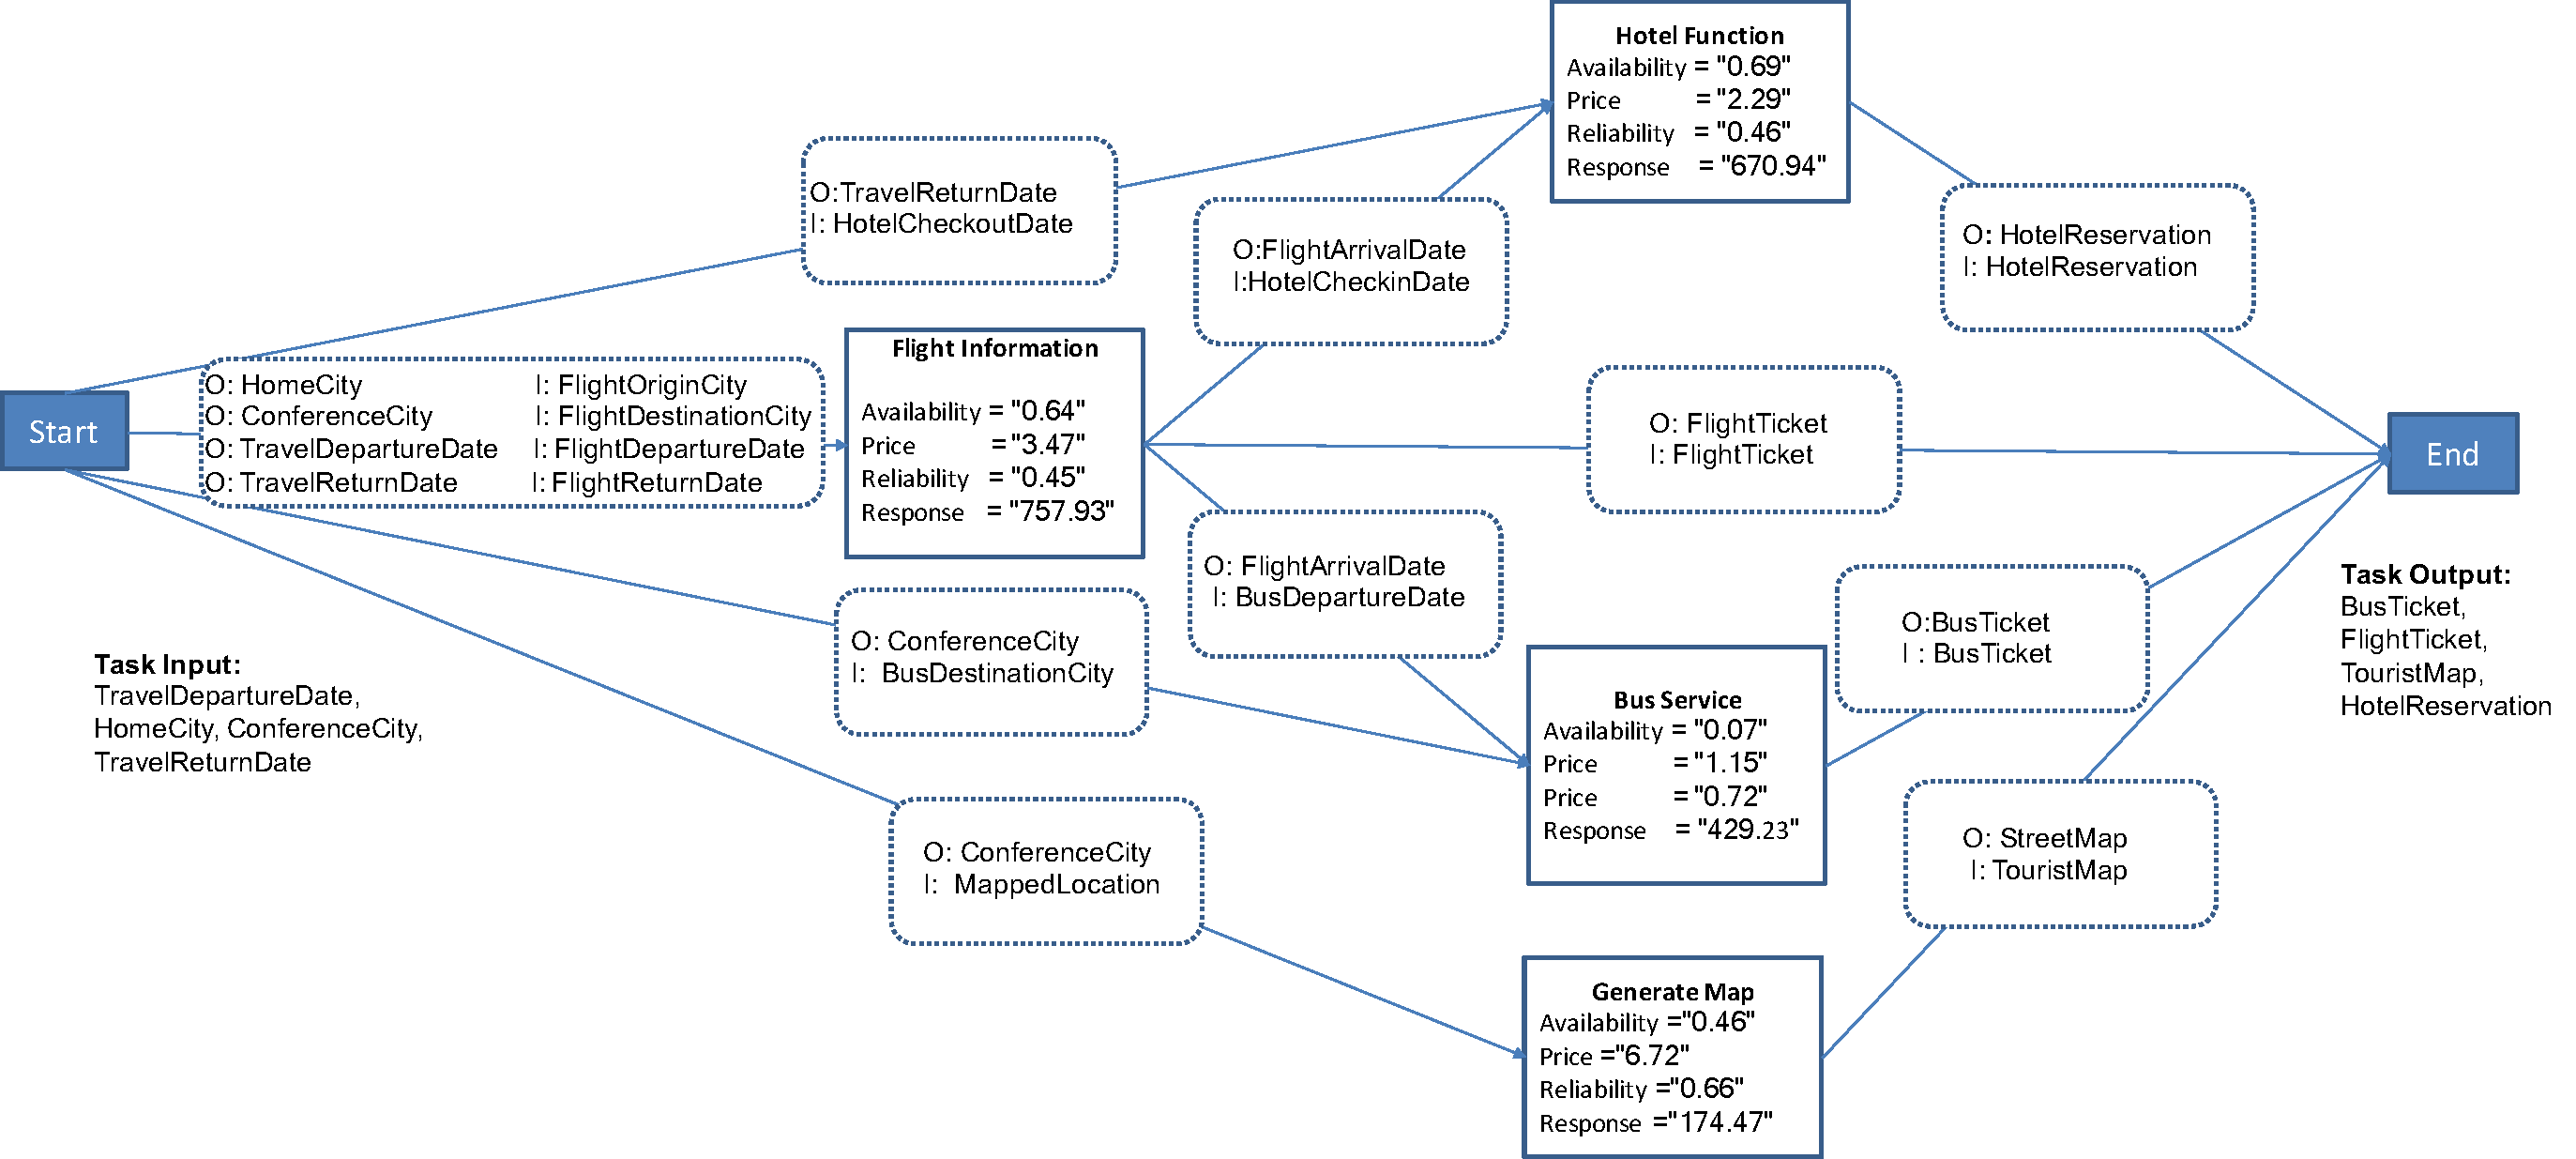
\includegraphics[scale=.25]{motivation.pdf}}
 \caption{ An example of a web service composition}
 \label{motivation}
\end{figure}QoS-aware web service composition \cite{da2016particle,da2015graphevol,yu2013adaptive,ma2015hybrid}

Although obtaining a correct combination of web service is essential, there are many ways to chain web services to reach users' needs with different web services from a service repository. These web services have different QoS in terms of different availability, price, reliability and response time. Moreover, valid semantic matches between two web services could also have different matchmaking quality. For example, Generate Map service produce StreetMap which is considered to be a valid semantic match to TouristMap from users' perspectives. These perspectives are captured in a taxonomy Fig .\ref{taxonomy}, where all the inputs and the outputs related to the web services are described for a travel planning domain. For example, the concept Map and its sub-concept urbanMap are assigned with a touristMap instance and streetMap instance respectively in Fig .\ref{taxonomy}. The valid semantic match is considered that an instance of urban Map can be an instance of Map, but not vice versa. However, if a web service $GenerateTouristMap$ is found in the service repository that produces TouristMap as an output, but price is "16.87". I consider its semantic matchmaking quality is higher than the service $GenerateMap$, but price negatively contributes to the overall QoS. Therefore, automatically generating solutions in considering both QoS and matchmaking quality is a very challenging problem.  

\begin{figure}[h]
\centering
\fbox{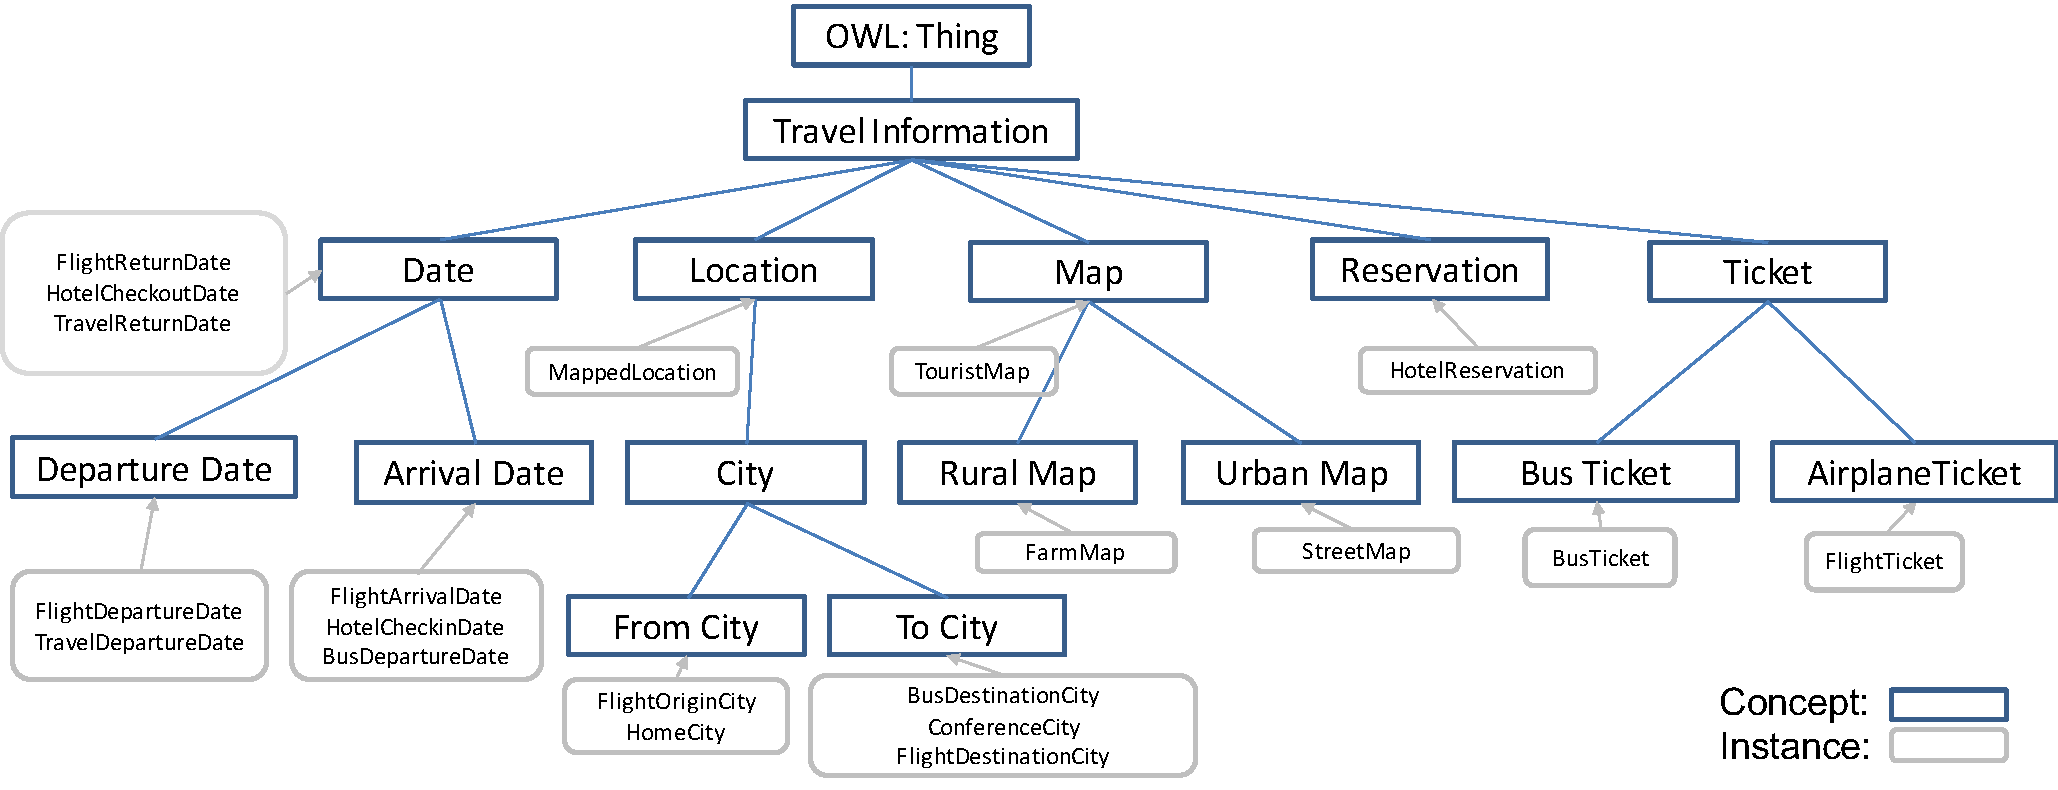
\includegraphics[scale=.28]{taxonomy.pdf}}
 \caption{ A taxonomy of a travel planning domain}
 \label{taxonomy}
\end{figure}

\subsection{Problem Formulation}\label{Motivation}

We herein give formal definitions of the assumptions the concepts regarding the semantic web service composition problem utilised in our approach that consists of four main concepts: a semantic web service model, a semantic matchmaking model, a weighted DAG composition model, and QoS calculation model, and composition problem model.
\vspace{0.3cm}

\textbf{Semantic Web Service Model}. The semantic web service model represents web services with functional descriptions, and how interoperability of web services enables matchmaking for automatically generating composition solutions.QoS-aware web service composition \cite{da2016particle,da2015graphevol,yu2013adaptive,ma2015hybrid}

\textbf{Definition 1.} A request from users is defined as a composition task in a tuple: $Comp.T = \{I_{T}, O_{T}\}$ by giving a set of task inputs $I_{T}$ and expecting  a set of desired task outputs $O_{T}$, where $I_{T}$ and $O_{T}$ are associated with related concepts $I^{C}_{T}$ and $O^{C}_{T}$ respectively in an ontology $O = \{(C, Taxonomy) \mid I^{C}_{T}, O^{C}_{T}  \subseteq C \}$.

\textbf{Definition 2.} A semantic web service is defined as a tuple $S = \{ I_{S}, O_{S}, QoS_S \}$ $\in$ $\mathcal{SR}$, where $I_{S}$ is a set of service inputs that must be satisfied to invoke $S$, and $O_{S}$ is a set of service outputs returned by the execution of $S$. $I_{S}$ and $O_{S}$ are concept-related instances that are linked to the concepts $I^{C}_{S}$ and $O^{C}_{S}$, where $ I^{C}_{S}, O^{C}_{S}  \subseteq C$. $QoS_S = \{ t_s, c_s, r_s, a_s, ... \} $ is a set of non-functional attributes of $S$, it typically refers to response time $t_s$, cost $c_s$, reliability $r_s$, and availability $a_s$ \cite{zeng2003quality}. $\mathcal{SR}$ is a service repository consisting of a set of $S$, where all the $S$ are registered.
\vspace{0.3cm}

\textbf{Semantic Matchmaking Model}. The mechanism to compose web services relays on the semantic descriptions of inputs and outputs, which enable inputs of a service to be matched by outputs of another. To measure the quality of these matches, we utilise different matchmaking types (\textit{exact, plugin subsumes and fail} \cite{paolucci2002semantic} ) into consideration for exploiting the semantics of inputs and outputs.

\textbf{Definition 3.} Given $a, b \in C$, $type(a, b)$ returns the matchmaking types of two concepts, and this matchmaking type is determined by the logic described in the $O$. If both $a$ and $b$ are equivalent, $exact$ type ($a \equiv b$) is returned. If the concept of $a$ is a sub-concept of the concept of $b$ type ($a \sqsubseteq b$) is returned. If the concept of $a$ is a super-concept of the concept of $b$, $subsumes$ type ($a \sqsupseteq b$) is returned. If none of previous matchmaking types are returned, $fail$ type ($a \perp b$) is returned.

We use the $type(a, b)$ to define full matchmaking between two concept-related input and output of two services.

\textbf{Definition 4.} Given $(a \in O^{C}_{S_m}) \vee (b \in I^{C}_{S_n}) \wedge (m \neq n) $, a $full match(a \Rightarrow b)$ holds if $type(a, b)$ returns $exact$ or $plugin$. The operator ``$ \Rightarrow$'' means $a$ is passed to $b$, and $b$ is fully satisfied by $a$. The full match is a guarantee of completely valid  ``$ \Rightarrow$'' operation, whereas, partial matches are not considered in this paper.

\textbf{Definition 5.} Given $full match(a \Rightarrow b)$, $q(a \Rightarrow b)$ is a function that given a output-related concept of a service and a input-related concept of another service, it returns the concept similarities between them.
\vspace{0.3cm}

\textbf{Weighted DAG Composition Model}. web service composition is considered to be a data workflow, where services are chained together by their inputs and outputs using the two models defined before. Naturally, all these concepts can be captured in a weighted DAG as $WG = (V, E)$ , where:

$V=\{Start, S1, S2...Sn, End\}$ is a set of services, where $Start$ and $End$ are two special services defined as $Start = \{ \phi, I_T, \phi \}$ and $End  = \{ O_T, \phi, \phi \}$. 

$E = \{e_{1}, e_{2},... e_{m} \}$ is a set of edges, where each edge has a set of incoming outputs $O_{S_{src}}$ from source service $S_{src}$ and a set of outgoing inputs $I_{S_{src}}$ from target service $S_{tar}$. 

$e = \{ (O_{S_{src}} \cup I_{S_{src}}) \mid \forall o \in O_{S_{src}}, \exists i \in O_{S_{src}} \wedge fullmatch (o \Rightarrow i) \}$
\vspace{0.5cm}

\textbf{QoS Model in a Weighted DAG}
Four most often considered QoS parameters \cite{zeng2003quality} are response time, cost, reliability and availability described as follows:\textit{Response time} ($T$) measures the expected delay in seconds between the moment when a request is sent and the moment when the results are received.\textit{Cost} ($C$) is the amount of money that a service requester has to pay for executing the web service. \textit{Reliability} ($R$) is the probability that a request is correctly responded within the maximum expected time frame. \textit{Availability} ($A$) is the probability that a web service is accessible. The aggregation value of QoS in a DAG respect to the structures of DAG, which reflects how services associated with each other in a service composition. The QoS calculation models are described as follows:


\textbf{Definition 6.} $V_{A}(WG)$ is a function that given a $WG$, a aggregated $availability$ value is returned defined as :
$V_{A}(WG)=\prod\limits^n_{k=1}a_k$, for all $\{S_1, S_2, ... S_n\} \subset V$.

\textbf{Definition 7.} $V_{R}(WG)$ is a function that given a $WG$, a aggregated $reliability$ value is returned defined as :
$V_{R}(WG)=\prod\limits^n_{k=1}r_k$, for all $\{S_1, S_2, ... S_n\} \subset V$.

\textbf{Definition 8.} $V_{C}(WG)$ is a function that given a $WG$, a aggregated cost value is returned defined as :
$V_{C}(WG)=\sum\limits^n_{k=1}c_k$, for all $\{S_1, S_2, ... S_n\} \subset V$.


\textbf{Definition 9.} $V_{T}(WG)$ is a function that given a $WG$, a aggregated time value is returned, where  $T$ is determined by the most time-consuming path in the composition flow of the solution, which is defined as :
$V_{T}(WG)$ $=MAX\{timePath(WG)_n$ $|n\in\{1,\ldots,m\}\}$, where m is the number of $timePath$.

\vspace{0.5cm}

\textbf{Composition Problem}
A set of semantic web services $S$ are chained as a weighted DAG composition model $WG$ when a composition task $Comp.T$ is requested by users. The composition problem considered in this paper to automatically generate $WG$, satisfying the follows:

$\forall WG^{'}$ , $\{q(a \Rightarrow b) \} \cup V_{A}(WG^{'}) \cup V_{R}(WG^{'}) \cup V_{C}(WG^{'}) \cup V_{T}(WG^{'})  \leq \{ q(a \Rightarrow b) \} \cup V_{A}(WG) \cup V_{R}(WG) \cup V_{C}(WG) \cup V_{T}(WG) $ 





\section{Comprehensive Quality Model}\label{Comprehensive_Quality_Model}
In this section, we propose a general comprehensive quality-aware service model in consideration of both semantic matchmaking quality and QoS for semantic web service composition. This model overcome the disadvantages of current prevailing QoS-aware quality model that ignores quality of semantic matchmaking.


\subsection{Comprehensive Quality Model}\label{qualityModel}

\textbf{Semantic web Service link}. In Fig. \ref{semanticLink}, $S_{1}$ and $S_{2}$ are linked to together if exists any parameter matchmaking between  Output of $S_1$ and Input of $S_2$.  Therefore, measuring semantic matchmaking quality ($SM$) is to measure the overall quality of semantic web service link ($sm_{L}$), which is aggregated from the quality of parameter matchmaking ($sm_{P}$). This semantic web service link is adopt from \cite{lecue2009optimizing}.

\begin{figure}[h]
\centering
\fbox{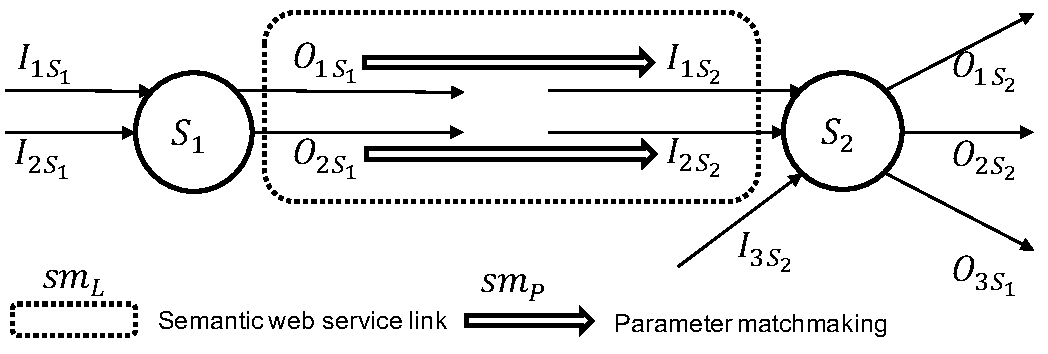
\includegraphics[scale=.38]{semanticLink.pdf}}
 \caption{ An example of semantic web service link}
 \label{semanticLink}
\end{figure}


\textbf{Semantic web matchmaking quality model}. Due to that the discretisational characteristics of different match types and values assigned to matching types are driven by the cost of data integration and manipulation \cite{lecue2009optimizing}, partial ordering match types are considered to be one factor for quality of parameter matchmaking, denoted as $mt_{p}$,  For example, Exact matching type demands less time for computation compared to that of Plugin match. Another factor in our proposed model is concept similarity, which could be evaluated based on the edge counting method defined in \cite{shet2012new}. This formula (\ref{equation1}) is used to estimate the concept similarity between matching parameters, which is denoted as $s_{p}$. N1 and N2 measure the distances from an output-related concept and an input-related concept to the top node of a taxonomy respectively, and N measure the distances from the closest common ancestor of these two matched input-related and output-related concepts. $\lambda$ is set to 0 if we do not measure the similarities of neighbourhood concepts that is not the matching levels considered in this paper. Consequently, given the quality of parameter matchmaking type and quality of parameter concept similarity, the quality of parameter matchmaking is defined by Formula (\ref{equation2}).

\begin{equation}
s_{p}{=} \frac{2N \cdot e^{-\lambda L/D} }{N_{1}+N_{2}}
\label{equation1}
\end{equation}

\begin{equation}
\label{equation2}
sm_{p} \stackrel{.}{=} (mt_ {p}, \  s_ {p})
\end{equation}

Further more, since semantic web service link represent services connections, where quality of semantic web service link $(sm_{L})$ is considered to be semantic matching quality on service level by the aggregation of parameter matchmaking quality. Therefore, $sm_{L}$ is defined in formula (\ref{equation3}), where $sm_{L}$ and $s_{L}$ are the average value of all involved $mt_{p}$ and $s_{p}$ respectively. 

\begin{equation}
\label{equation3}
sm_{L} \stackrel{.}{=} (mt_ {L}, \  s_ {L})
\end{equation}

\textbf{Comprehensive quality model}. The comprehensive quality model consider both semantic matchmaking quality and QoS. The semantic matchmaking quality refers to $sm_{L}$. Consequently, the comprehensive quality model is defined in Formula (\ref{equation4}), which could be further broken down into Formula (\ref{equation5}). 
\begin{equation}
\label{equation4}
cq \stackrel{.}{=} (sm_ {L}, \  QoS_ {s})
\end{equation}
\begin{equation}
\label{equation5}
cq \stackrel{.}{=} (mt_ {L}, \  s_ {L}, \  a_{s},\  r_{s},\  c_{s},\  t_{s})
\end{equation}

\textbf{Semantic matchmaking quality aggregation}. The quality aggregation is defined based on the constructs of composition web services in consideration of semantic matchmaking quality and QoS. The quality on composition solution is further calculated by following the formula (\ref{equation6})(\ref{equation7}), and QoS aggregation are discussed in Sect. \ref{Quality of Service and Composition Constructs}

\begin{equation}
\label{equation6}
MT {=} \prod_{n=1}^{m} mt_ {L_{n}}
\end{equation}
\begin{equation}
\label{equation7}
S {=} (\sum_{n=1}^m s_ {L_{n}})/m
\end{equation}


\subsection{Objective Function}
In real life, given a unique and optimised solution is always easier for customers to pick up directly when many quality criteria involved into decision making, rather than provided a set of solutions. It is very practical to define a single fitness as a weighted sum of all the quality related components in Formula (\ref{equation8}). Note that weights can be adjusted according to users' preferences. The function value of 1 means the best comprehensive quality and 0 means the worst. For this purpose, $MT$, $S$, $A$, $R$, $T$, and $C$ must be normalised so that the function value falls within the range from 0 to 1 using Formula (\ref{equation9}) and (\ref{equation10}), where the maximum and minimum value of $A$, $R$, $T$, and $C$ are calculated by all web services related to the composition task. $MT$ and $S$ are using a bound from 0 to 1. Therefore, the composition task is try to find maximised value of objective function associated to the solutions.

\vspace{-0.2cm}
\begin{equation}
\label{equation8}
Fitness = w_1 \hat{MT} + w_2 \hat{S} + w_3 \hat{A} + w_4 \hat{R} + w_5(1 - \hat{T}) + w_6(1 - \hat{C})
\end{equation}
\noindent where $\sum_{i=1}^{6} w_i = 1$
\\
\vspace{-0.2cm}
\begin{equation}
\label{equation9}
\hat{Q_k} = 
\begin{cases}
	\frac{Q_k - Q_{k, min}}{Q_{k, max} - Q_{k, min}} & \text{ if }Q_{k, max} - Q_{k, min} \neq 0.\\
	1 & \mathrm{ otherwise}.
\end{cases}
\end{equation}
\noindent where $k$ $=$ $1$, $2$, $3$, and $4$, where $Q_1$ is $MT$, $Q_2$ is $S$, $Q_3$ is $A$, and $Q_4$ is $R$.
\begin{equation}
\label{equation10}
\hat{Q_j} = 
\begin{cases}
	\frac{Q_{j,max} - Q_j}{Q_{j, max} - Q_{j, min}} & \text{ if }Q_{j, max} - Q_{j, min} \neq 0.\\
	1 & \mathrm{ otherwise}.
\end{cases}
\end{equation}
\noindent where $j$ $=$ $1$, and $2$, where $Q_1$ is $T$ and $Q_2$ is $C$.


Our comprehensive quality evaluation model is considered to be more general. Semantic matchmaking types (Exact and Plugin) are considered for discovering desired web service in QoS-aware web service composition  \cite{ma2015hybrid,da2016particle,da2015graphevol}, but there are no measurements of matchmaking types and concept similarities. Consequently, weights for $MT$ and $S$ are considered to be 0 in our propopsed comprehensive evaluation model, it turns to a widely used QoS evaluation model in \cite{ma2015hybrid,da2016particle,da2015graphevol}.
\section{PSO-based Approach to Comprehensive Quality-Aware Automated Semantic Web Service Composition}\label{qswsc_approach}

\begin{figure*}[h]
\centering
\fbox{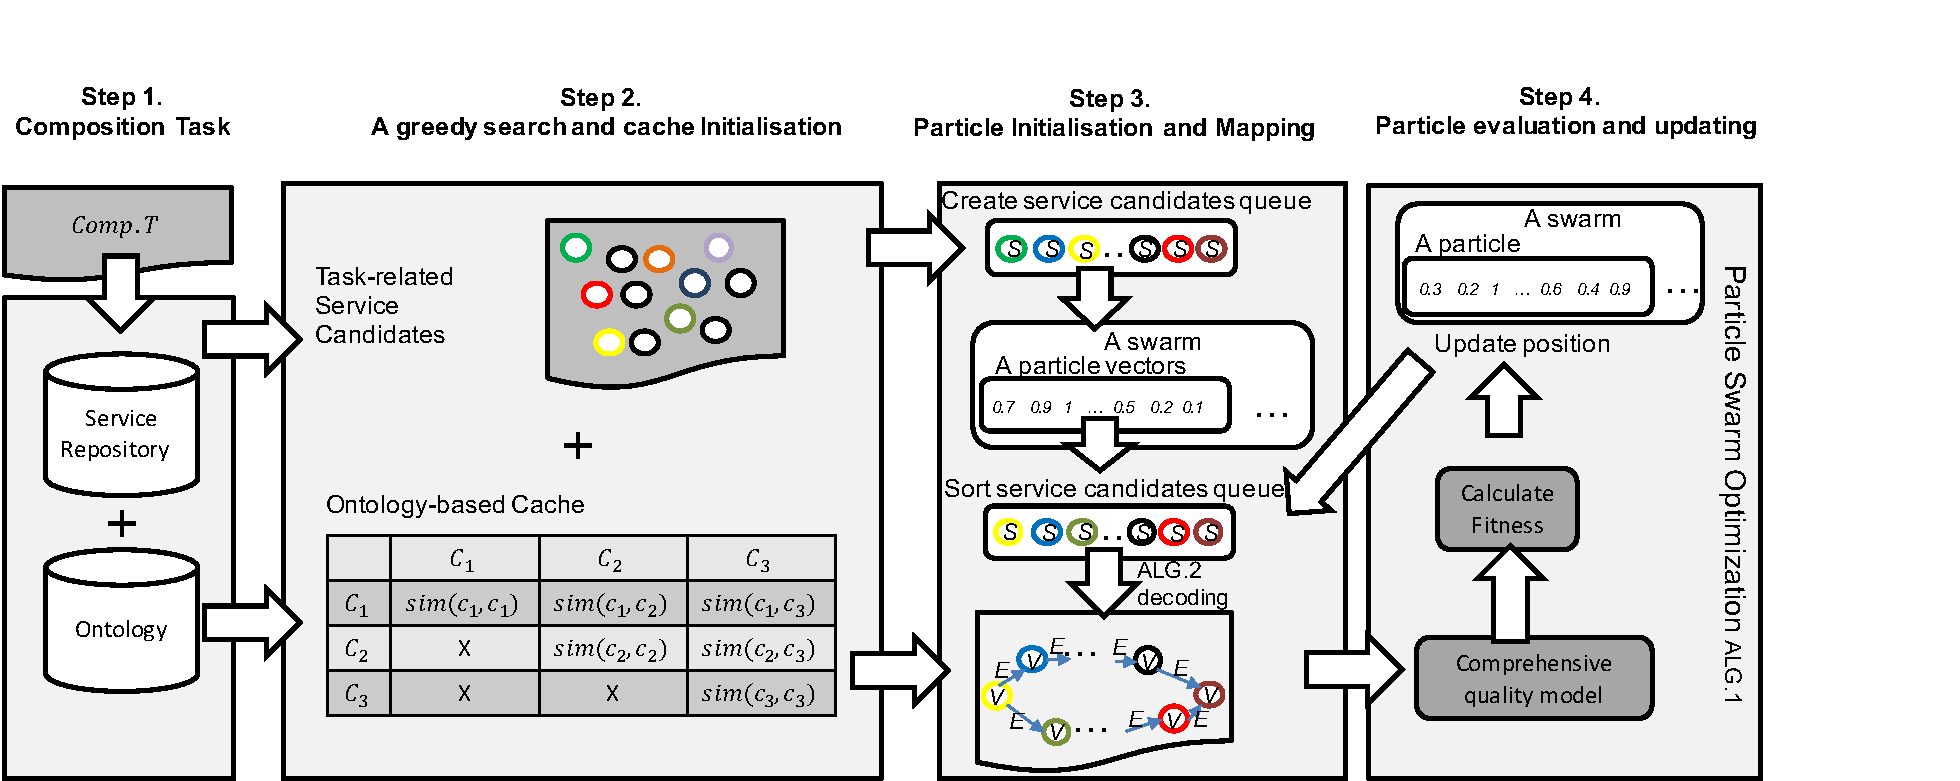
\includegraphics[scale=.4]{overview.pdf}}
 \caption{Overview of POS-based approach to QoS-aware automated semantic web service composition.}
 \label{overview}
\end{figure*}


\subsection{PSO-based Approach to QoS-Aware Semantic Web Service Composition}

PSO has shown its efficiency in solving combinatorial optimisation problems \cite{fukuyama2008fundamentals}. Therefore, we will employ a PSO-based approach, which is considered to be easier to maintain the correctness of solutions compared to GP-based approaches that often require repairing or penalising the solutions \cite{da2016particle}. Fig. \ref{overview} shows the overview of our approach with five steps. Step 1: The composition process is triggered by a composition goal defined in Subsection \ref{problemDes}, which describes customers requirements both semantic matchmaking quality and QoS. Step 2: This composition goal are used to discover all relevant web services, which lead to a shrunken service repository that is subsequently used by PSO as a searching space. Step 3: A weighted graph representation is randomly built up from an initial service queue that mapped to the particle's location, interleaving with semantic matchmaking process utilising ontology-based index cache. In the weighted graph, graph edges are assigned with semantic matchmaking quality as weights. Step 4: The fitness value of the weighted graph is evaluated to update the position of particle under PSO algorithm in Sect. \ref{pso_algorithm}, where the position is mapped to the index of service queue. later on, the updated service queue is used to decode a new weighted graph as the composition solution. Step 5. Lastly, the best position found in the searching space is selected and decode into the final optimised solution. This PSO-based approach is similar to \cite{da2016particle}, but we employ weighted graphs as a different solution presentation with explicit support for the proposed quality model.


\subsection{Ontology-based Index Cached Optimisation}\label{indexCache}
our PSO-based approach demands decoding processes from optimised queues to weighted DAGs, the bottlenecks of efficiently generating weighted DAGs lie in building edges and nodes, which are related to the cost of semantic quality calculation and the size of service repository respectively. To effectively construct weighted DAGs, we pre-calculate semantic matchmaking quality. The key idea of the index is to create a map using a pair of keys, output-related concepts and potentially matched input-related concepts with considering different levels of match types, and the map values stored $mt_{p}$ and $mt_{s}$. Meanwhile, this index size could also be reduced by only considering the concepts related in the shrunken service repository, which means the index cache is filtered by those task-relevant web services. This optimised cache also contributes to less and constant time for weighted graphs building through the whole evolutionary process.


\subsection{QoS-aware Semantic Web Service Composition Algorithm} \label{pso_algorithm}


\begin{algorithm}
 \setlength\hsize{0.9\linewidth}
 \SetKwInOut{Input}{Input}\SetKwInOut{Output}{Output}
 \SetKwFunction{generateWeightedGraph}{generateWeightedGraph}
 \SetKwProg{Procedure}{Procedure}{}{}
 \LinesNumbered
 \SetNlSty{}{}{:}
 \Input{relevant Web services $rws$}
 \Output{Optimised service queue $queue$,Optimised Weighted Graph $OPTWG$}
 Map each relevant service to an index in the particle's position vector\;https://www.facebook.com/
 Randomly initialise each particle in the swarm\;
  \While {max. iterations not met}{
     \ForEach{particles in the swarm}{
     $queue \leftarrow$ map service in a descending order by particle's position vector\;
     $WG \leftarrow$ $generateWeightedGraph$()\;
	 Calculate the $WG$ fitness value\;
     
      \eIf{fitness value better than \emph{pBest}}{    
        Assign current fitness as new \emph{pBest}\;
       }{
        Keep previous \emph{pBest}\;
       }	
     }
    Assign best particle's \emph{pBest} value to \emph{gBest}, if better than \emph{gBest}\;
 	Calculate the velocity of each particle\;
  	Update the position of each particle\;
  }
 \KwRet $OPTWG$\;
 \caption{Steps of the PSO-based Web service composition technique.}
\label{novelSteps}
\end{algorithm} 


\begin{algorithm}
 \setlength\hsize{0.9\linewidth}
 \SetKwInOut{Input}{Input}\SetKwInOut{Output}{Output}
 \SetKwFunction{generateWeightedGraph}{generateWeightedGraph}
 \SetKwProg{Procedure}{Procedure}{}{}
 \LinesNumbered
 \SetNlSty{}{}{:}
  \Procedure{\generateWeightedGraph{}}{
 \Input{Task inputs $I$, task outputs $O$, Optimised service queue $queue$, IndexCache $IndexCache$}
 \Output{Weighted Graph $WG$}
 $WG \leftarrow  null$\;
 $WG \leftarrow$ new $endNode$(), new $startNode$()\;
 $OutputSet \leftarrow$ \{$I$\}\;
  \While {all $O$ $\notin$ $OutputSet$  and $queue !=null$}{
     \ForEach{$ws$ in $queue$}{
      \uIf{$ws.inputs$ $\in$ $OutputSet$ }{    
    		 \ForEach{$I$ in $ws.inputs$}{
    		$mt_{P}, s_{P} \leftarrow$ query $IndexCache$\;
     		$mt_{L} \leftarrow$ aggregation($mt_{p}$)\;
 			$s_{L} \leftarrow$ aggregation($s_{p}$)\;
              }
        $sm_{L} \leftarrow$ \{ $mt_{L}$,$s_{L}$ \}\;
        $WG.edge \leftarrow$  $sm_{L} $\;
        $WG \leftarrow$ new $wsNode$()\;
         $OutputSet$ add \{$ws.outputs$\}\;    
       $queue$.remove $ws$\;
       }	
     }
  }
 remove $dangling nodes$\; 
 remove $dangling edges$\;
 \KwRet $WG$\;
 }
 \caption{Create a composition weighted graph from a queue.}
\label{graph_building}
\end{algorithm} 


The overall algorithm investigated here is made up of the PSO-based web service composition algorithm \ref{novelSteps} and the decoding algorithm \ref{graph_building}. In algorithm \ref{novelSteps}, the idea is to translate the particle location produced by PSO into a service queue as an indirect representation, such that finding the best fitness of the weighted graph is to discover the optimised location of the particle in the search space. In PSO, the dimension of each particle equals to the number of relevant web services. The index of each services is mapped to a separate location component in a particle. Then services queue is sorted by the particles' position vector in the ascending order, from which we decode a weighted graph using Algorithm \ref{graph_building}. It is a simple forward graph building algorithm, and this method can lead to more services and edges connected to the graph that must be removed. Also, semantic quality value are assigned to all the edges, which is calculated from quality aggregation function with given parameter matchmaking quality.


\section{Experiment Design}\label{experiment_design}
In this section, a quantitative evaluation approach is adopted in our experiment design. The objectives of the evaluation are to $(1)$ measure the effectiveness of the comprehensive quality model in automated semantic web service composition approach; and $(2)$ compare solutions generated by a recent QoS-ware evaluation approach \cite{ma2015hybrid,da2016genetic} with our evaluation method proposed in the paper; and $(3)$ compare our PSP-based method with one existing GP-based approach \cite{ma2015hybrid}.


We utilise benchmark dataset web service challenge 2009 (WSC09) \cite{kona2009wsc} to perform the evaluation. WSC09 provides problems with five tasks corresponding to variable number of services, and ontologies. Therefore, it is a challenge dataset for measuring the scalability of our quality evaluation model. Table \ref{wsc09datasetTable} presents the features of the WSC’09 dataset. The number of concepts, individuals in the ontology and services in each data set is shown in the second, third, fourth column respectively. Also, we extend all the datasets with QoS attributes from service providers to enable our evaluation. 

\begin{table}[]
\centering
\caption{Features of the WSC09 datasets}
\label{wsc09datasetTable}
\begin{tabular}{l|l|l|l}
\hline
\multicolumn{1}{c|}{Dataset} & No.Concept & No.Individual & No.Service \\ \hline
WSC09 01                     & 1578       &3102           &572      \\ \hline
WSC09 02                     & 12388      &24815          &4129      \\ \hline
WSC09 03                     & 18573      &37316          &8138      \\ \hline
WSC09 04                     & 18673      &37324          &8301      \\ \hline
WSC09 05                     & 31044      &62132          &15211    \\ \hline
\end{tabular}
\end{table}

The parameters were chosen based on general settings from \cite{shi2001particle} for our PSO-based approach, In particular, PSO population size is 30 with 100 generations. We run 30 times independently for each dataset. We configure weight of fitness function to properly balance functional side and nonfunctional side. Therefore, $w_{1}$ and $w_{2}$ are set equally to 0.25, and $w_{3}$, $w_{4}$, $w_{5}$, $w_{6}$ are all set to 0.125 accordingly. The $mt_{p}$ is set to 1 (Exact match) and 0.75 (Plugin). In general, weight settings and parameter match type quality are decided by users' preferences.


\section{Results and Analysis}\label{results_analysis}
\subsection{Comparison Test for Comprehensive Quality Evaluation Model and QoS Evaluation Model}\label{comparisonTest}

A recent widely used QoS Evaluation Model, $QoS = w_1 \hat{A} + w_2 \hat{R} + w_3(1 - \hat{T}) + w_4(1 - \hat{C})$, where $\sum_{i=1}^{4} w_i = 1$, is used for QoS-aware web service composition \cite{ma2015hybrid,da2016particle,da2015graphevol}. We employ this QoS evluation model and our proposed comprehensive quality evluation model using our proposed PSO-based approach for searching for optimal solutions.
To analyse the differences in optimal solutions found by these two evaluation model, we recorded and compared the different mean values of $MT$, $S$, $QoS$ at the 100th generation over 30 runs. To make a sense of the comparison, all these recorded values are normalised from 0 to 1, and compared using statistical analysis in in Table \ref{decisionTable}. 

We observe an interesting pattern from Table \ref{decisionTable}. The mean values of $QoS$ using QoS evaluation model are significantly higher than those using comprehensive quality evaluation model for Task 2, 3, 4 and 5,  but the mean value of $MT$ and $S$ using comprehensive quality evaluation model are consistently significantly higher than those using QoS evluation model for all tasks with a slight trade-off in $QoS$.

\begin{table}[]
\footnotesize
\centering
\caption{Mean values of $MT$, $S$, and $QoS$ for QoS Evaluation Model and Comprehensive Quality Evaluation Model using PSO-based approach}
\label{decisionTable}
\begin{tabular}{l|l|l|l}
\hline
\multicolumn{2}{c|}{WSC09}              & QoS Evaluation Model         &\shortstack{Comprehensive \\ Quality Evaluation Model} \\ \hline
\multirow{3}{*}{Task1}  &$MT$   &0.189787 $\pm$ 0.039278686            &0.221862 $\pm$ 0.009582 $\uparrow$ \\ \cline{2-4} 
                        &$S$    &0.884962 $\pm$ 0.014140               &0.894082 $\pm$ 0.009206 $\uparrow$ \\ \cline{2-4}
                        &$QoS$  &0.278730 $\pm$ 0.007786               &0.280222 $\pm$ 0.008212                          \\ \hline
\multirow{3}{*}{Task2}  &$MT$   &0.001795 $\pm$ 0.000719               &0.001977 $\pm$ 0.001566 $\uparrow$ \\ \cline{2-4} 
                        &$S$    &0.906971 $\pm$ 0.005855               &0.923970 $\pm$ 0.006898 $\uparrow$   \\ \cline{2-4}
                        &$QoS$  &0.239979 $\pm$ 0.000578 $\uparrow$    &0.238596 $\pm$ 0.001264 \\ \hline
\multirow{3}{*}{Task3}  &$MT$   &0.158526 $\pm$ 0.014028               &0.245830 $\pm$ 0.007761 $\uparrow$   \\ \cline{2-4} 
                        &$S$    &0.949109 $\pm$ 0.002331               &0.972765 $\pm$ 0.002980 $\uparrow$           \\ \cline{2-4}
                        &$QoS$  &0.247002 $\pm$ 0.000661 $\uparrow$    &0.245631 $\pm$ 0.000431            \\ \hline
\multirow{3}{*}{Task4}  &$MT$   &0.000000 $\pm$ 0.000000               &0.000004 $\pm$ 0.000002 $\uparrow$ \\ \cline{2-4} 
                        &$S$    &0.879514 $\pm$ 0.007456               &0.920733 $\pm$ 0.000001 $\uparrow$ \\ \cline{2-4}
                        &$QoS$  &0.242297 $\pm$ 0.000507 $\uparrow$    &0.236677 $\pm$ 0.002211  \\ \hline
\multirow{3}{*}{Task5}  &$MT$   &  0.000042 $\pm$ 0.000030             &0.000078 $\pm$ 0.000020 $\uparrow$           \\ \cline{2-4} 
                        &$S$    &  0.915933 $\pm$ 0.012888             &0.927678 $\pm$ 0.002578 $\uparrow$                 \\ \cline{2-4}
                        &$QoS$  & 0.238189 $\pm$ 0.000240 $\uparrow$   &  0.237485 $\pm$  0.000328  \\ \hline                                                   
\end{tabular}
\end{table}

To better understand a better semantic matchmaking quality with a slight trade-off in the opitmal solutions using comprehensive quality evaluation model, we demonstrate the optimal solutions using task 3 as an example. Fig. \ref{comparisontest} $(1)$ and $(2)$ show two weighted DAGs as best solutions found by employing QoS-aware approach and Comprehensive quality-aware method respectively. Two approaches generate exactly the same service workflow structure, but some service vertices and edges denoted in red are different. To better understand these differences, we list the overall semantic matchmaking quality $SM$,  overall $QoS$ and semantic matchmaking quality associated to each edge ($sm_{e_1}$ to $sm_{e_4}$) for the two weighted DAGs in Fig. \ref{comparisontest} $(3)$, where $\Delta Q$ reveals the gain (positive $\Delta Q$) or loss (negative $\Delta Q$) for the listed qualities using our comprehensive quality evalutaion model. Therefore, an overall gain 0.1433 is calculated from a sum of $SM$ gain (0.1467) and $QoS$ loss (-0.0034). Consequently, our comprehensive evaluation model acheive a desirable trade-off in considering both semantic matchmaking and QoS. To demonstrate the value of semantic matchmking gain, we pick up $e_4$ associated with a smallest $\Delta Q$, where edeges $e_4$ to $WG(1)$ using QoS evaluation model and $WG(2)$ using comprehensive quality model have two different source service vertices $Ser1640238160$ and $Ser1947554374$ respectively,  and the same $end$ vertices. $Ser1640238160$ and $Ser1947554374$ are services with concept-related output parameters $Inst795998200$ and $Inst582785907$ corresponds to two concepts $Con103314376$ and $Con2037585750$ respectively marked on the related taxonomy in Fig. \ref{comparisontest} $(4)$. These two services $Ser1640238160$ and $Ser1947554374$ are associated with concept-related output parameters $Inst795998200$ and $Inst582785907$, and these parameters  are corresponds to two concepts $Con103314376$ and $Con2037585750$ respectively marked on the related taxonomy in Fig. \ref{comparisontest} $(4)$. In addtion, $Inst658772240$ are the required parameter for the $end$ vertice, which is related to concept $Con2113572083$. There exist $Inst582785907$ $\in$ $Con2037585750$ $\sqsubseteq_{3}$ $Inst658772240$ $\in$ $Con2113572083$ for $e_4$ in $WG(1)$ and $Inst795998200$ $\in$ $Con103314376$ $\sqsubseteq_{2}$ $Inst658772240$ $\in$ $Con2113572083$ for $e_4$ in $WG(2)$. Therefore, 2-levels Subsumes is closer 3-level Subsumes, $Inst795998200$ is closer to user's required outputs $Inst658772240$ compared with $Inst582785907$.

\begin{figure}[h]
\centering{
\fbox{
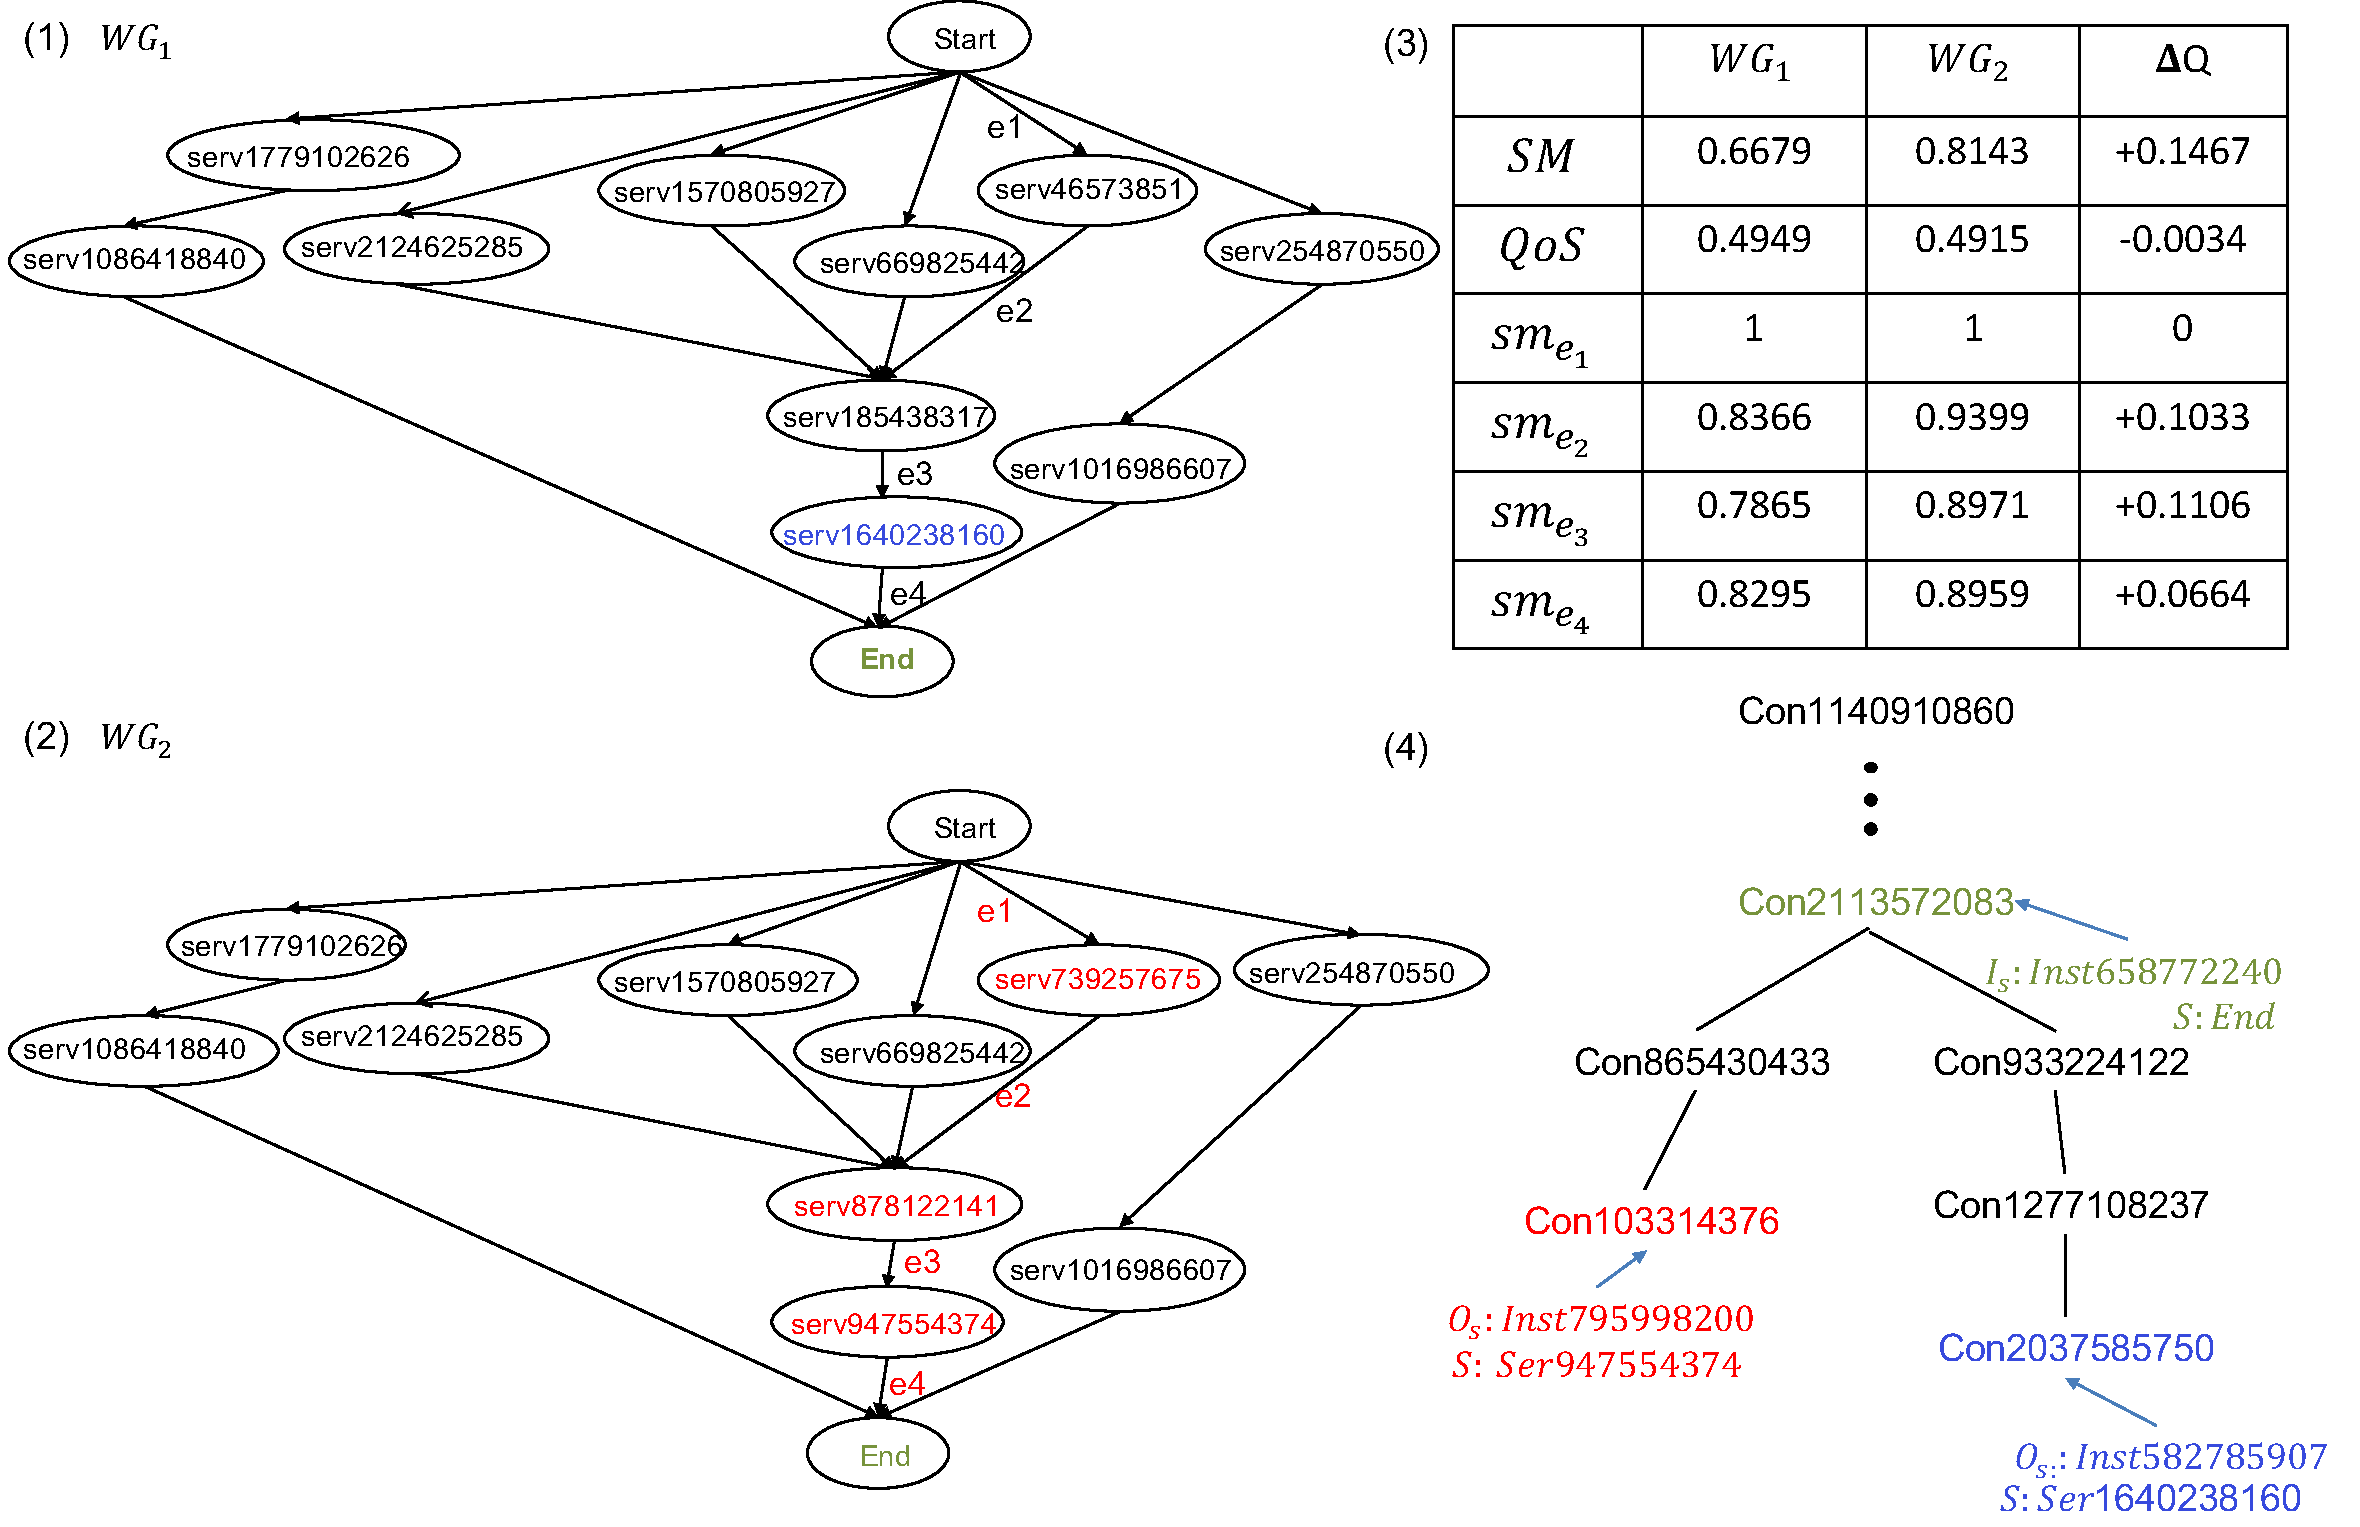
\includegraphics[scale=.22]{comparisontest.pdf}}}
 \caption{Example Comparison of solutions to Task 3 using two different evaluation model.}
 \label{comparisontest}
\end{figure}

\subsection{Comparison Test with GP-based approach}\label{comparisonTestWithGP}
To evaluate the performance of our proposed PSO-based approach, we compare one GP-based approach  \cite{ma2015hybrid} with our PSO method. we consider the links between child nodes and parent nodes as semantic web service links for measuring  semantic matchmaking quality, and those links information are maintained correctly for the crossover and mutation. Therefore, we evaluate both semantic matchmaking quality and QoS simultaneously using the proposed comprehensive quality model. To make a fair comparison with our PSO-based, we consider the same number of evaluations (3000 times) as that in our PSO-based approach, we set the parameters settings for GP-based approach \cite{ma2015hybrid} using 30 individuals and 100 generations.

The Table \ref{meanFitness} shows the mean fitness values accomplished by two methods. We employ statistical analysis to test the significant differences in mean fitness value. The results show that the PSO-based approach performs better in four of five tasks (all the p-values are consistently smaller than 0.01).

\begin{table}[]
\centering
\caption{Mean fitness results for comparing GP-based approach}
\label{meanFitness}
\begin{tabular}{l|l|l}
\hline
\multicolumn{1}{c|}{Dataset} & PSO-based approach & GP-based approach  \\ \hline
WSC09 01                     &0.559207 $\pm$ 0.012780  $\uparrow$   &0.520659 $\pm$ 0.020758           \\ \hline
WSC09 02                     &0.470083 $\pm$  0.001106 $\uparrow$   &0.459681 $\pm$  0.002874          \\ \hline
WSC09 03                     & 0.550396 $\pm$ 0.012780                        &0.567915 $\pm$ 0.023447 $\uparrow$   \\ \hline
WSC09 04                     & 0.468942 $\pm$ 0.001670  $\uparrow$   &0.431704 $\pm$ 0.009774            \\ \hline
WSC09 05                     & 0.469424 $\pm$ 0.000800  $\uparrow$   &0.245222 $\pm$ 0.036885            \\ \hline
\end{tabular}
\end{table}

At last, We also compare the average fitness value with optimum through the evolutionary process for both two approaches over 30 independent runs. Fig. \ref{psovsgp} is an example of convergence rate for Task 3, where the behaviour of PSO-based approach presents a very clear evidence of fast convergence and reaches a better-optimised solution, while the performance of GP is barely satisfactory, as GP-based method improves its fitness value gradually.


\begin{figure}[h]
\centering
\fbox{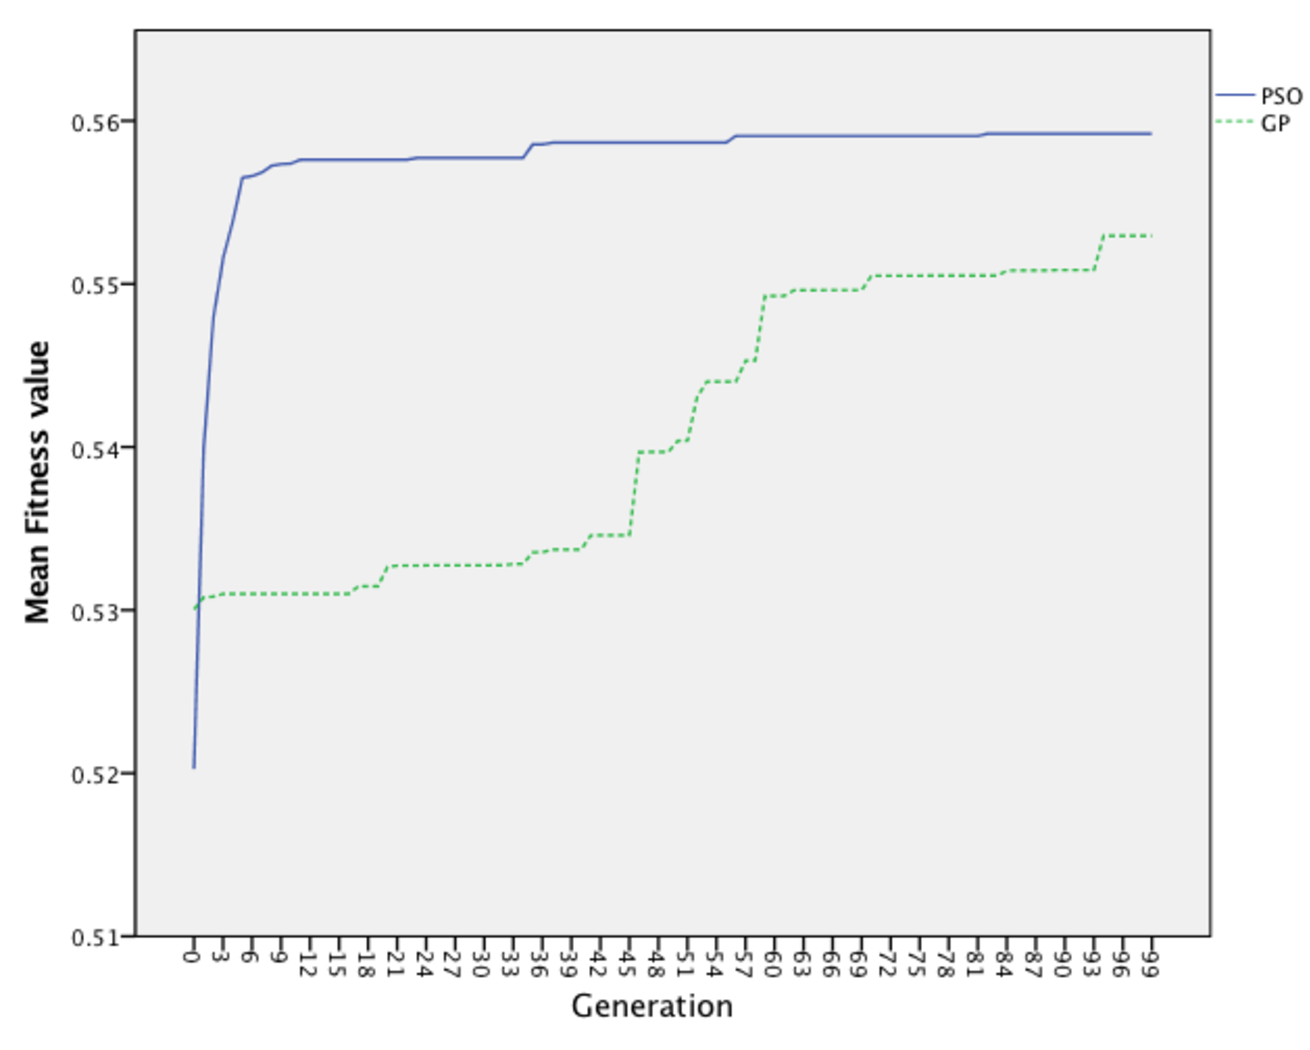
\includegraphics[scale=.25]{psovsgp.pdf}}
 \caption{An example of comparing convergency rate of PSO and GP approaches for task 3}
 \label{psovsgp}
\end{figure}



\section{Conclusion}\label{conclusion}
This work introduces a general comprehensive evaluation model for considering semantic matchmaking quality and QoS. We proposed a PSO-based service composition approach utilising our proposed quality mode that can achieve a desired balance of both quality aspects. Also, we compare one GP-approach with our PSO-based method to show our performance results in finding more optimised solution. Future works can investigate multi-objective EC techniques to produce a set of composition solutions for the situations when the quality preference is not known.


\bibliographystyle{splncs03}
\bibliography{IEEEexample}

\end{document}